\chapter{Derivation of State Machine Models from Process Models\label{chapter:deductive}}

This chapter shows how state machines can be synthesised from process models. They capture the trace semantics of process models, making them amenable to formal analysis such as model-checking.

\section{Motivation}

\section{Introducing guarded transition systems}

This section introduces guarded LTS (g-LTS) as an intermediate formalism between guarded hMSCs and LTS. Roughly, a g-LTS is a transition system with guards or events on transitions. It provides a convenient milestone on the way from a guarded hMSC to the corresponding LTS, in particular, for determining the set of traces accepted by the guarded hMSC. As a structured form of LTS, a g-LTS representation avoids state explosion. It is easier to understand and facilitates code generation. Moreover, interresting analyses may be performed at g-LTS level, see \cite{Damas:2011}.

\begin{definition}[Guarded LTS]
\noindent A guarded LTS is defined as a structure $(Q,\Sigma,\Phi,\delta,q_{0},C_{0})$ where 
\begin{itemize}
\item $Q$ is a finite set of states,
\item $\Sigma$ is a set of event labels, 
\item $\Phi$ is a set of fluents defined on $\Sigma$,
\item $\delta$ is a transition relation $Q \times \Sigma_{\tau}\cup\mathcal{P}(2^\Phi) \times Q$,
\item $q_{0} \in Q$ is the initial state,
\item $C_{0} \in \mathcal{P}(2^\Phi)$ is an initial condition. 
\end{itemize}
\end{definition}

In a guarded LTS, transitions are labeled either by a guard or by an event. Non-observable $\tau$-transitions are also allowed; their usage is the same as in pure LTS. 

A guard is a propositional formula over fluents in $\Phi$. The set of such formula is denoted by $\mathcal{P}(2^\Phi)$, as in Section \ref{section:background-fluents}. Intuitively, the guard must be evaluated to true for its transition to be activated. This is made precise is the next section.

The condition $C_0$ plays the same role as in guarded hMSCs. It is a boolean formula that constraints the acceptable initial values of fluents. 

\subsection{Trace semantics\label{subsection:glts-trace-semantics}} 

The semantics of g-LTS is defined in terms of event traces involving no guards at all.

\begin{definition}[g-LTS execution]
An \emph{execution} of a g-LTS $G = (Q,\Sigma,\Phi,\\\delta,q_{0},C_{0})$ from $q_0$ is a pair $(Init, \textless l_0, \ldots,l_n\textgreater)$, where 
\begin{itemize}
\item $Init \in 2^\Phi$ is an initial fluent value assignment, mapping every fluent in $\Phi$ to true or false,
\item $\textless l_0,\ldots,l_n \textgreater$ is an finite sequence of labels $l_i \in \Sigma_{\tau}\cup\mathcal{P}(2^\Phi)$, some of them being event labels (including $\tau$) and others being guards.
\end{itemize}
\end{definition}

Only certain executions are considered valid from the initial state of the g-LTS. This is captured by the following definition:

\begin{definition}[Valid g-LTS execution]
An execution $S = (Init,\textless l_0,\ldots,l_n\textgreater)$ of a g-LTS $G = (Q,\Sigma,\Phi,\delta,q_{0},C_{0})$ is \emph{valid} from its initial state $q_0$ iif the following \emph{acceptance conditions} are met for every $i$ such that $0 \leqslant i < n$:\\
\vspace{-0.8cm}
\begin{tabbing}
\indent trace inclusion:~~~~~~~\= $\exists q_{i+1} \in Q$ such that $(q_i,l_i,q_{i+1}) \in \delta$\\
\indent admissible start:      \> $Init \models C_0$ \\
\indent guard satisfaction:    \> $S_i \models l_i$ if $l_i \in \mathcal{P}(2^\Phi)$\\
\end{tabbing}
\vspace{-0.8cm}
where $S_i$ is the fluent value assignment after the i-th event in the trace, with $S_0 = Init$.
\end{definition}

The first condition states that the label sequence denotes an existing path in the automaton. The second condition states that the initial fluent value assignment must meet the initial condition $C_0$. The third condition ensures that all guards are met along the sequence.

The trace semantics of a g-LTS is defined as a set of event traces. Roughly, it consists of all valid executions where $\tau$ labels as well as guards have been removed. This is precisely captured by the the following definition.

\begin{definition}[g-LTS trace semantics]
The set of traces accepted by a g-LTS $G = (Q,\Sigma,\Phi,\delta,q_{0},C_{0})$ is defined as:
\begin{align*}
\mathcal{L}(G) &= \{~w|_{\Sigma} \mid \exists~Init \in 2^\Phi~s.t.~(Init,w)~is~a~valid~execution~for~G~\}
\end{align*}
\end{definition}

Section \ref{subsection:from-glts-to-lts} provides a composition algorithm to capture this set of traces through a pure LTS, that is, a LTS with event labels only. The next section will first refine the LTS hiding and composition operators defined in Section \ref{section:background-state-machines} to handle guards.

\subsection{Hiding and composition in presence of guards}

The hiding operator on g-LTSs is very similar to the one on LTSs, defined in Section \ref{subsection:lts-hiding}. 

\begin{definition}[g-LTS hiding]
The \emph{hiding} of a set of labels $I$ in a g-LTS $G = (Q,\Sigma,\Phi,\delta,q_{0},C_{0})$ defines the g-LTS
\begin{equation*}
G \setminus I = (Q,\Sigma \setminus I,\Phi,\delta_{hidden},q_{0},C_0)
\end{equation*}
\noindent where $\delta_{hidden}$ is the smallest relation satisfying the following rules:
\begin{center}
\begin{tabular}{cc}
$\frac{\displaystyle G \stackrel{l}{\longrightarrow} G'}{\displaystyle G \setminus I \stackrel{l}{\longrightarrow} G' \setminus I}~~l \notin I$ & 
$\frac{\displaystyle G \stackrel{l}{\longrightarrow} G'}{\displaystyle G \setminus I \stackrel{\tau}{\longrightarrow} G' \setminus I}~~l \in I$ \\
\end{tabular}
\end{center}
\end{definition}

As with LTSs, the hiding operator makes a set of labels invisible by replacing them by $\tau$ transitions. Note that the definition above allows hiding both guards and events. 

The special case where $I = \mathcal{P}(2^\Phi)$ yields a g-LTS with no guard remaining. In this case, we will consider that the hiding operator actually returns a LTS defined as follows:
\begin{equation*}
G \setminus \mathcal{P}(2^\Phi) = (Q,\Sigma,\delta_{hidden},q_0)
\end{equation*}

We also define a composition operator on g-LTS, as follows:

\begin{definition}[g-LTS composition]
Let $G = (Q_1,\Sigma_1,\Phi_1,\delta_1,q_{1},C_{1})$ and $H = (Q_2,\Sigma_2,\Phi_2,\delta_2,q_{2},C_{2})$ denote two g-LTS. Their \emph{composition} is another g-LTS 
\begin{equation*}
G \parallel H = (S_1 \times S_2,\Sigma_1\cup\Sigma_2,\Phi_1\cup\Phi_2,\delta,(q_1,q_2),C_1 \wedge C_2)
\end{equation*}
\noindent where $\delta$ is the smallest relation satisfying the following rules:

\centering
\begin{tabular}{cl}
$\frac{\displaystyle G \stackrel{l}{\longrightarrow} G'}{\displaystyle G \parallel H \stackrel{l}{\longrightarrow} G' \parallel H}$ & $l \notin \mathcal{P}(2^\Phi)$, $l \notin \Sigma_2$ \\[20pt]

$\frac{\displaystyle H \stackrel{l}{\longrightarrow} H'}{\displaystyle G \parallel H \stackrel{l}{\longrightarrow} G \parallel H'}$ & $l \notin \mathcal{P}(2^\Phi)$, $l \notin \Sigma_1$ \\[20pt]

$\frac{\displaystyle G \stackrel{l}{\longrightarrow} G',~H \stackrel{l}{\longrightarrow} H'}{\displaystyle G \parallel H \stackrel{l}{\longrightarrow} G' \parallel H'}$ & $l \notin \mathcal{P}(2^\Phi)$, $l \neq \tau$ \\[20pt]

$\frac{\displaystyle G \stackrel{g}{\longrightarrow} G',~H \stackrel{h}{\longrightarrow} H'}{\displaystyle G \parallel H \stackrel{g \wedge h}{\longrightarrow} G' \parallel H'}$ & $g \in \mathcal{P}(2^{\Phi_1})$, $h \in \mathcal{P}(2^{\Phi_2})$, $g \wedge h \nvDash false$ 
\end{tabular}
\end{definition}

The first three rules are the same as with LTS composition (see Section \ref{subsection:lts-composition}); they explicitly exclude guards here. The last rule states that the two LTSs must transit on guards together, provided that their conjunction is satisfiable. The resulting transition is then labeled with this conjunction.

\section{From guarded hMSC to pure LTS}

\subsection{From guarded hMSC to guarded LTS}

A guarded hMSC can be rewritten as a g-LTS. The latter abstracts from the agents and captures the set of global behaviors covered by the g-hMSC. The rewriting algorithm extends the technique presented in Section \ref{subsection:background-hmsc} that synthesizes a LTS capturing the traces of hMSC \cite{Uchitel:2004}. The algorithm may
be outlined as detailed below. It is illustrated in Fig.~\ref{image:scheduler-ghmsc-glts} for the guarded hMSC in Fig.~\ref{image:scheduler-ghmsc}.

\begin{description}
\item[Handling nodes] Every hMSC node yields a behaviorally equivalent sub-LTS.
\begin{itemize}
\item A MSC node is rewritten as a sub-LTS collecting the linear event sequences from the scenario. For a MSC $M$, the LTS captures the set of traces $\mathcal{L}_{total}(M)$ defined in Section \ref{subsection:background-positive-scenarios}.
\item For a node expanded into a finer-grained hMSC, the procedure is applied recursively to obtain the corresponding sub-LTS.
\item A decision node is rewritten as a sub-LTS having only one state and no event; the same applies to the start and end nodes of the hMSC.
\end{itemize}
In the first two cases, the $Task_{start}$ and $Task_{end}$ special events are added to the corresponding sub-LTS.
\item[Handling edges] The edges in a guarded hMSC yield transitions between the terminal and initial states of the sub-LTS corresponding to their source and target nodes, respectively.
\begin{itemize}
\item An outgoing edge of a decision node is labeled by a guard and yields a guarded transition in the g-LTS.
\item Any other edge is simply converted as a $\tau$ transition.
\end{itemize}
\end{description}

\begin{figure}[H]\centering
\scalebox{0.60}{
  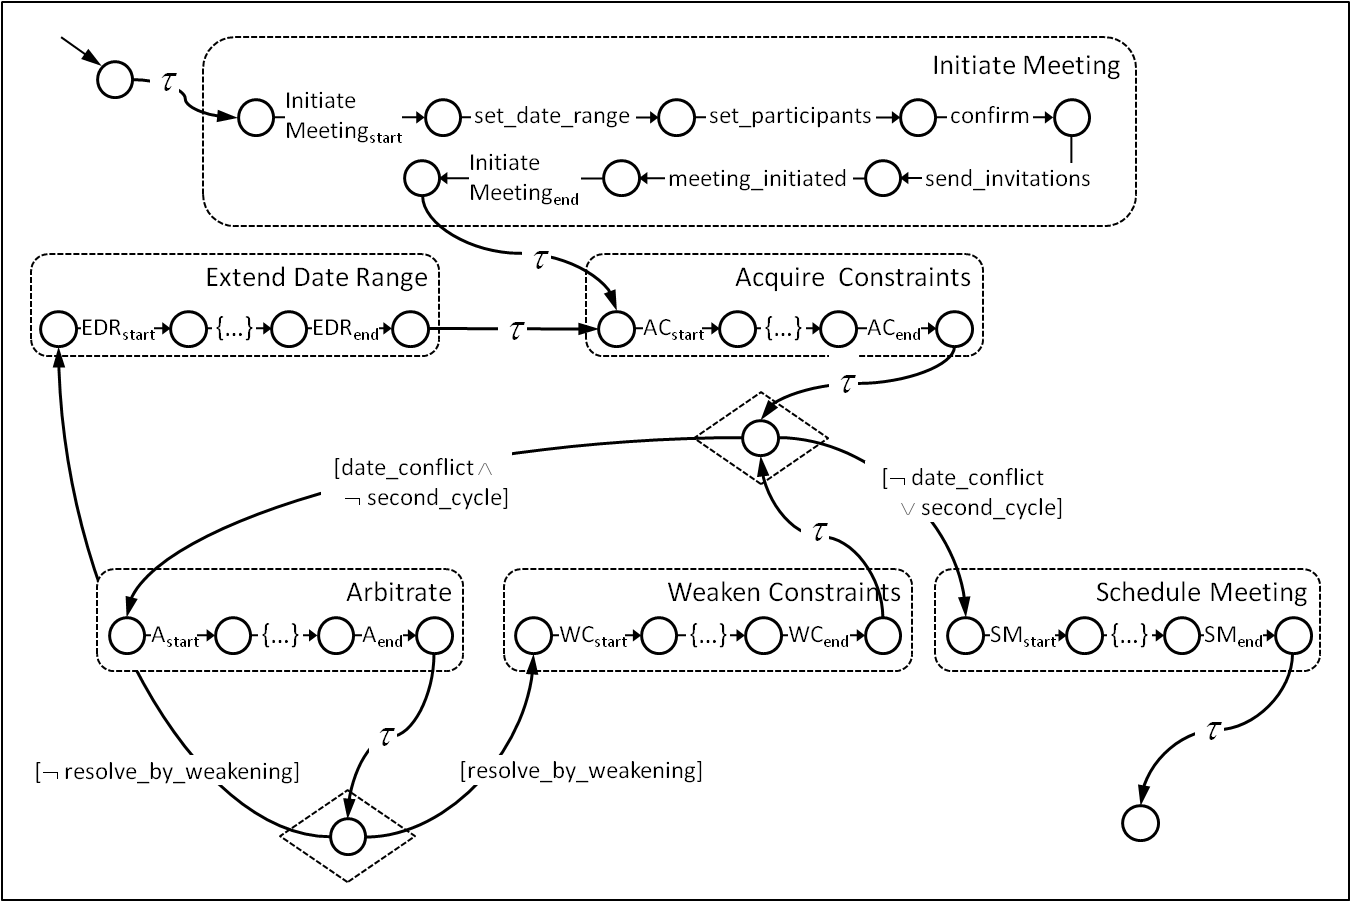
\includegraphics[trim=2mm 2mm 2mm 2mm, clip]{src/3-deductive/images/ghmsc-glts-scheduler}
}
\caption{Rewriting a g-hMSC as a g-LTS, on the meeting scheduler process in Fig.~\ref{image:scheduler-ghmsc}.\label{image:scheduler-ghmsc-glts}}
\end{figure}

\subsection{From guarded LTS to pure LTS\label{subsection:from-glts-to-lts}}

The set of traces accepted by a g-LTS is determined by building a trace-equivalent LTS. For this, a parallel composition of g-LTSs if first computed so as to meet the various acceptance conditions in Section \ref{subsection:glts-trace-semantics}. The first g-LTS in this composition is a super g-LTS meeting the \emph{trace inclusion} and \emph{admissible start} condition. To meet the \emph{guard satisfaction} condition, the set of traces of the super g-LTS is pruned further by composing it with fluent automata. Let us make each of them in the composition further precise.

\noindent \textbf{Super g-LTS} -- By definition, the input g-LTS already meets the \emph{trace inclusion} condition. In order to meet the \emph{admissible start} condition, it is extended by converting the initial condition $C_0$ as an explicit guard from the initial state. 

Let denote the input g-LTS by $G = (Q,\Sigma,\Phi,\delta,q_{0},C_{0})$; the super LTS is defined as:
\begin{equation*}
Super~LTS = (Q \cup \{ q_{start} \}, \Sigma, \Phi, \delta \cup \{(q_{start},C_0,q_0)\},q_{start},true)
\end{equation*}

\noindent \textbf{Fluent g-LTS} -- The \emph{guard satisfaction} condition is enforced by pruning all traces violating guards in the super g-LTS. For this we compose the latter with fluent automata. The latter keep track of the current fluent values; guard events are constrained to happen only when the corresponding guard is true.

A fluent $Fl = \textless Init_{Fl}, Term_{Fl} \textgreater $ yields a g-LTS $G_{Fl} = (Q,\Sigma,\Phi,\delta,q_{0},C_{0})$ where
\begin{align*}
Q      &= \{q_u,q_t,q_f\}            \\
\Sigma &= Init_{Fl} \cup Term_{Fl}   \\
\Phi   &= \{ Fl \} \\
\delta &=    \{~(q_f,e,q_t) \mid e \in Init_{Fl}~\}~\cup \{~(q_t,e,q_t) \mid e \in Init_{Fl}~\} \\
       &\cup~\{~(q_t,e,q_f) \mid e \in Term_{Fl}~\} \cup \{~(q_f,e,q_f) \mid e \in Term_{Fl}~\} \\
       &\cup~\{~(q_u, [Fl], q_t),~(q_u, [\neg Fl], q_f)~\} \\
       &\cup~\{~(q_t, [Fl], q_t),~(q_f, [\neg Fl], q_f)~\} \\
q_0    &= q_u \\
C_0    &= true
\end{align*}

This resulting g-LTS is illustrated in Fig.~\ref{image:fluent-glts} for a generic fluent definition. A transition labeled with a set name between $\{$ and $\}$ brackets is a shortcut denoting one transition for each element of the set.

\begin{figure}[H]\centering
\scalebox{0.85}{
  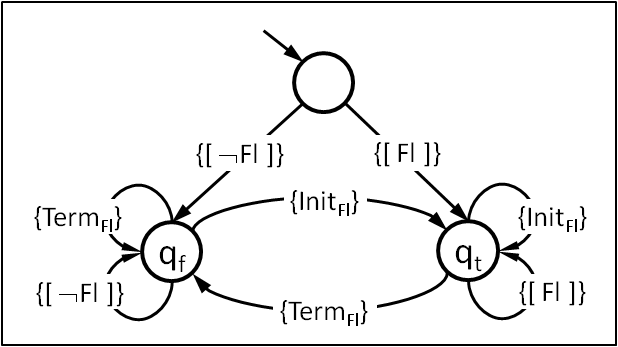
\includegraphics[trim=2mm 2mm 2mm 2mm, clip]{src/3-deductive/images/fluent-glts}
}
\caption{A generic fluent g-LTS\label{image:fluent-glts}}
\end{figure}

\noindent \textbf{Synthesized LTS} -- Putting pieces together, the trace-equivalent LTS of a g-LTS is obtained through the following computation:
\begin{align*}
\left((Super~LTS \parallel G_{Fl_1} \parallel \ldots \parallel G_{Fl_n}) \setminus \mathcal{P}(2^\Phi)\right)^\Delta
\end{align*}

That is, a g-LTS is first obtained through the composition of the Super LTS with fluent automata; all guards are then hidden, resulting in a pure LTS which can be further minimized.
